\part{Progettazione di un'interfaccia grafica per la compressione di immagini}

Abbiamo deciso di realizzare il software per la seconda parte del progetto utilizzando il framework Qt\cite{qt}, che permette di progettare interfacce grafiche scrivendo codice in linguaggio C++. Il nostro programma permette, fondamentalmente, di visualizzare, in tempo reale, il risultato di una compressione definiti il livello di taglio dei blocchi e la dimensione di quest'ultimi. Non è presente una funzionalità di salvataggio dell'immagine perché il nostro non è uno standard riconosciuto e sarebbe, per cui, inutilizzabile in altri programmi.
Idealmente, però, basterebbe progettare la struttura del file in modo da contenere le sequenze dei valori non nulli dei blocchi associata ad altre informazioni generali, come la dimensione reale dell'immagine, la grandezza dei blocchi o la soglia di taglio, per poter scrivere un visualizzatore di immagini che sia in grado di effettuare il parsing di quel file ed eseguire la IDCT2.

Il programma fornisce una schermata nella quale è possibile selezionare l'immagine da comprimere e i valori di compressione da applicare, ossia dimensione dei blocchi e la soglia di taglio delle frequenze. Nella parte sinistra della GUI viene mostrata l'immagine originale, mentre in quella di destra la sua versione compressa. In figura \ref{fig:deer} è riportato un esempio sull'immagine \textit{deer}, sulla quale sono stati applicati blocchi di elevate dimensioni (70x70) ed una elevata compressione (circa del 92\%), in questo modo è facilmente osservabile l'effetto della compressione sui blocchi e sull'immagine.

\begin{figure}[h]
	\centering
	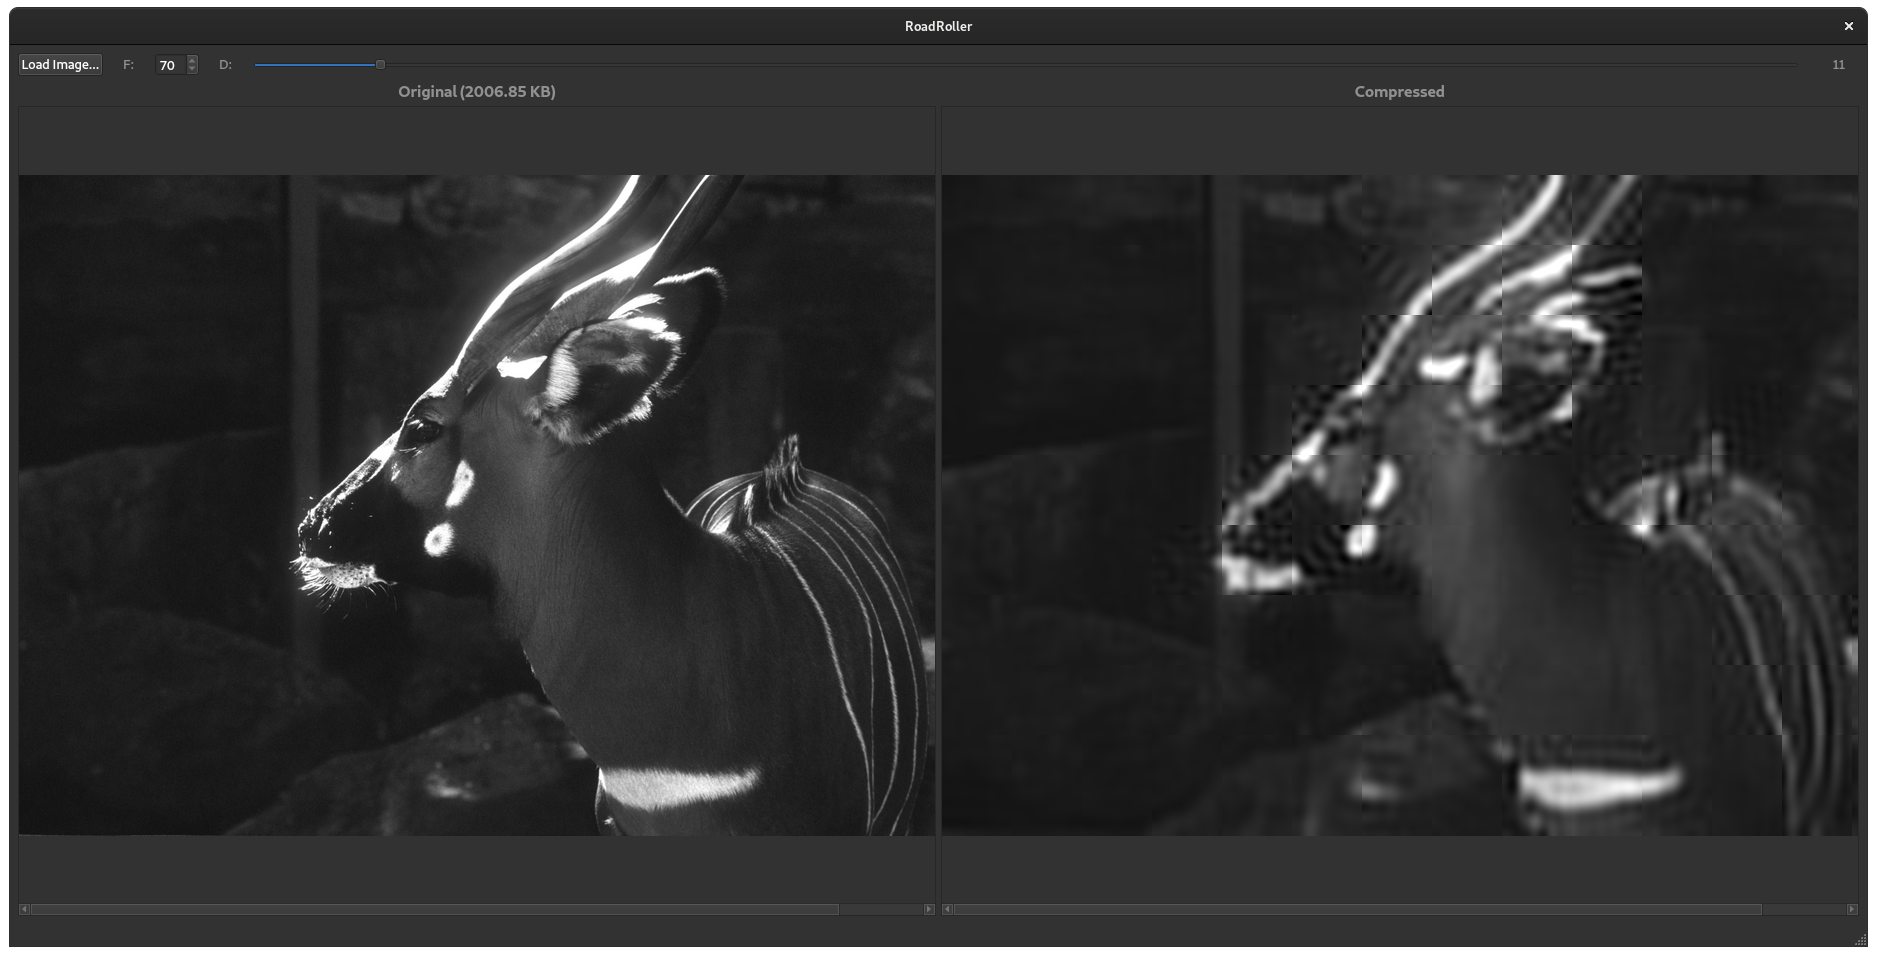
\includegraphics[width=1\linewidth]{figures/qt_deer}
	\caption{Programma di compressione basato su Qt}
	\label{fig:deer}
\end{figure}

Il diagramma delle classi relativo a questo progetto è molto breve, infatti sono state create solamente 2 classi. La prima per gestire l'interfaccia grafica, chiamata \textit{MainWindow}, mentre la seconda, \textit{BlockManager}, si occupa della gestione dei blocchi e la loro relativa compressione. In questo caso, a differenza del primo progetto, vi è meno la necessità di creare  un'architettura con più classi in quanto la funzionalità è unica e precisa. Abbiamo, comunque, fatto in modo che la classe relativa alla finestra GUI sia separata dalla logica di compressione delle immagini al fine di cercare di mantenere una certa \textit{separation of concerns}. Questo diagramma viene mostrato in Figura \ref{fig:class_diagram}.

\paragraph{Funzionamento della compressione e decompressione}
Abbiamo cercato di progettare la compressione in modo da renderla più efficiente possibile. In particolare, quando un'immagine viene caricata, viene predisposta un'area di memoria che rappresenta blocchi dell'immagine contigui. Essendo, però, i blocchi dell'immagine su pixel che non sono in realtà contigui, abbiamo creato un mapping che permette di capire a quale pixel dell'immagine corrisponde un certo blocco e viceversa. Con questa soluzione, abbiamo incrementato significativamente la performance in fase di caricamento dell'immagine, poiché invece di tante allocazioni quanti sono i blocchi ne viene richiesta solo una. Il parallelismo, inoltre, non è molto utile quando si effettuano allocazioni di memoria in quanto l'heap ha bisogno di essere gestito contro la concorrenza. Vedremo che, invece, il parallelismo è tornato molto utile in fase di compressione e decompressione.

\begin{figure}[h]
	\centering
	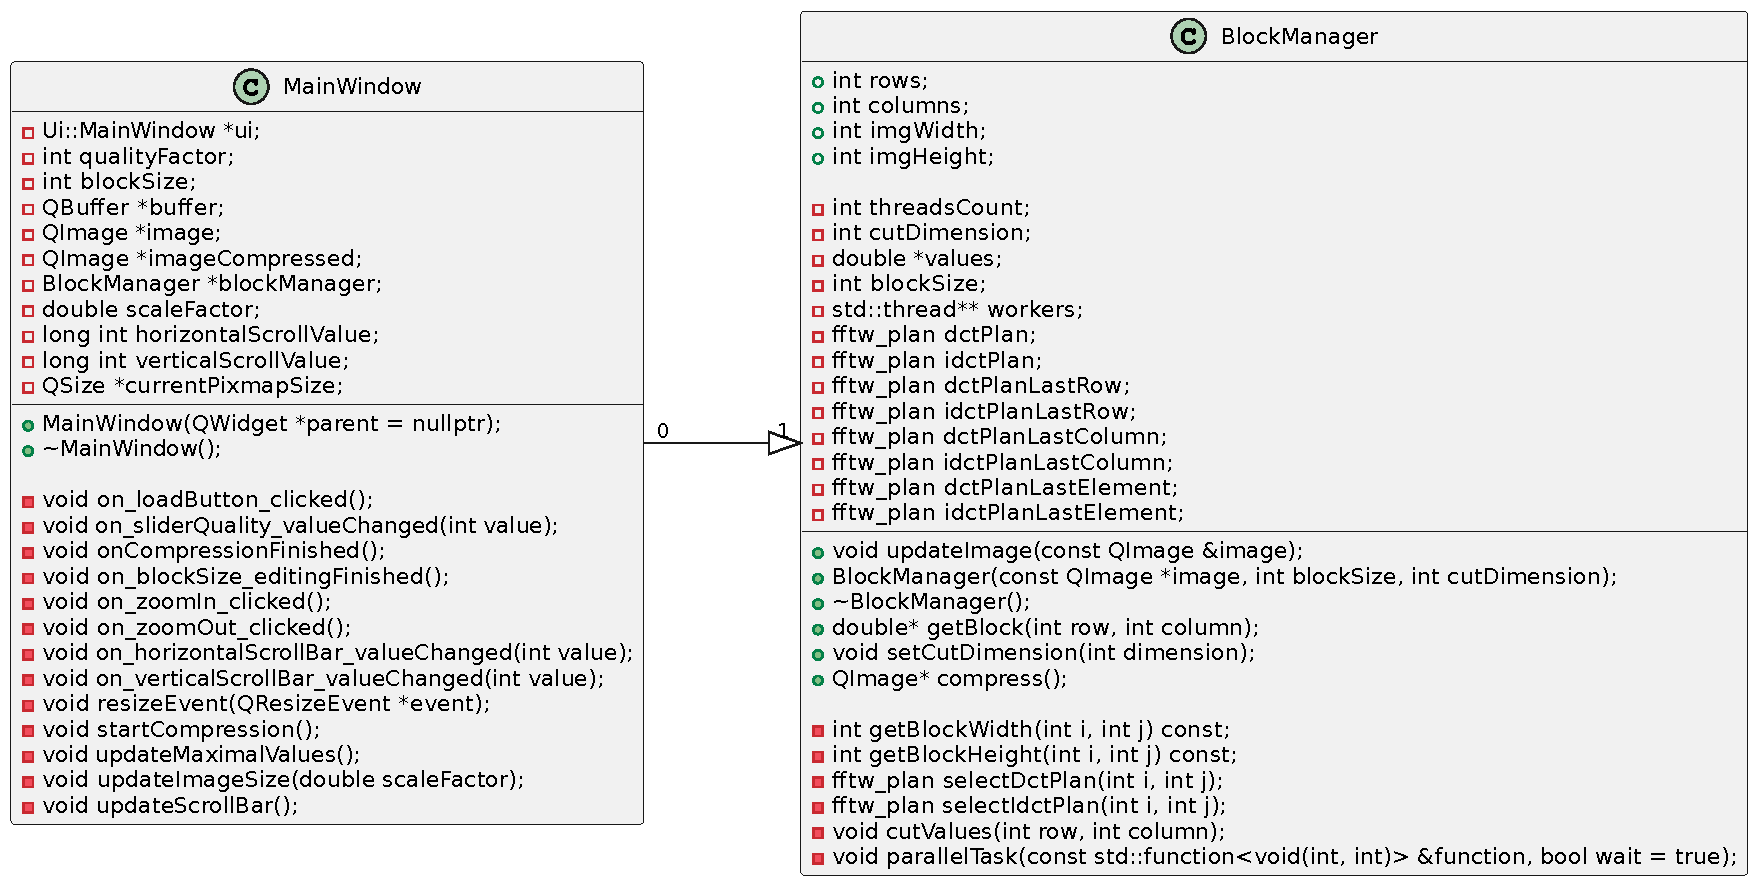
\includegraphics[width=1\linewidth]{figures/class diagram}
	\caption{Diagramma delle classi}
	\label{fig:class_diagram}
\end{figure}

\section{Features}

Alla versione base del progetto, descritto precedentemente, sono state aggiunte un insieme di funzionalità:

\begin{itemize}
	\item \textbf{Multithreading}: L'aggiunta dei thread permette una rapida compressione dell'immagine. Infatti essendo che i blocchi lavorano su aree della figura indipendenti gli uni dagli altri, è possibile eseguire le compressioni in parallelo, così come la scrittura dei pixel nell'oggetto immagine finale.
	
	Abbiamo fatto in modo che l'immagine venisse suddivisa in macroblocchi disgiunti tra loro, ognuno contenente un insieme di blocchi $F \times F$ dell'immagine. La cardinalità di questo insieme di macroblocchi è pari circa al numero di core/thread del processore su cui verrà eseguito il nostro programma di compressione. In questo modo, è possibile bilanciare il livello di parallelismo sulla base delle capacità della macchina di parallelizzare i task.
	\item \textbf{Navigazione dell'immagine}: All'interno dell'interfaccia grafica sono presenti degli slider e dei tasti per zoomare nelle immagini. Questi tasti sono sincronizzati in modo tale da poter visionare contemporaneamente le stesse zone delle 2 immagini. In questo modo si possono osservare più comodamente i vari effetti che la compressione comporta sulle immagini.
	\item \textbf{Aggiornamento in tempo reale}: Abbiamo costruito l'interfaccia grafica in modo che l'utente possa regolare e visualizzare in tempo reale la compressione dell'immagine, anche su zone particolari (ad esempio, dopo uno zoom). Grazie al parallelismo, inoltre, siamo riusciti a migliorare la latenza di questa operazione.
	\item  \textbf{Gestione dei bordi}:  A fini sperimentali, abbiamo provato ad implementare il processo di compressione in modo che venisse effettuata la DCT anche su blocchi di dimensioni inferiori, composti dagli scarti derivati dalla suddivisione in blocchi di dimensione $ F \times F$. Ulteriori informazioni su questa prova sono presenti alla Sezione \ref{sec:border}.
	
	\end{itemize}

\section{Gestione dei pixel in eccesso}\label{sec:border}

All'interno di questo progetto, abbiamo deciso in modo "sperimentale" di gestire in maniera leggermente diversa da jpeg i pixel sui margini.

Nello specifico, il nostro programma di compressione considera i pixel in eccesso derivati dalla suddivisione in blocchi e li utilizza per creare dei blocchi più piccoli, al fine di riempire l'intera immagine. Dopo questa operazione, ne esegue la DCT2 allo stesso modo degli altri blocchi. Prima di eseguire il taglio, però, la soglia di azzeramento delle frequenze viene adattata in modo da essere proporzionato alla minore quantità di frequenze e da rendere, quindi, la compressione dell'immagine più uniforme:

$$d' = \floor*{d  \sqrt{ \frac{W \cdot H}{F^{2}}}}$$

dove W e H rappresentano rispettivamente la larghezza e l'altezza del blocco preso in considerazione.
Inoltre, nel caso in cui $d'=0$, ma $d>0$, si mantiene il valore 1 al fine di evitare buchi indesiderati.

Abbiamo preso questa decisione perché, a differenza di jpeg, non siamo stati vincolati dalla matrice di quantizzazione e abbiamo potuto, quindi, sperimentare una gestione leggermente diversa del margine dell'immagine.


\begin{figure}
	\begin{minipage}{0.5\textwidth}
		\begin{center}
		
			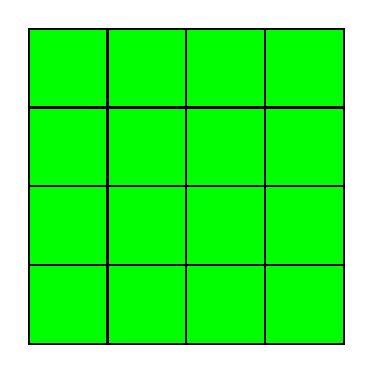
\begin{tikzpicture}
				[%%%%%%%%%%%%%%%%%%%%%%%%%%%%%%
				box/.style={rectangle,draw=black,thick, minimum size=1cm},
				]%%%%%%%%%%%%%%%%%%%%%%%%%%%%%%
				
				\foreach \x in {0,1,...,3}{
					\foreach \y in {0,1,...,3}
					\node[box, fill=red] at (\x,\y){};
				}
			
			
				\foreach \x in {0,...,3}{
					\foreach \y in {0,...,3} {
						\ifnumcomp{\x + (3 - \y)}{<}{5}{
							\node[box, fill=green] at (\x,\y){};
						}{};
					}
				}
				
				
			\end{tikzpicture}
		\end{center}
		\begin{center}
			(a)
		\end{center}
	\end{minipage}\hfill
	\begin{minipage}{0.5\textwidth}
		\begin{center}
			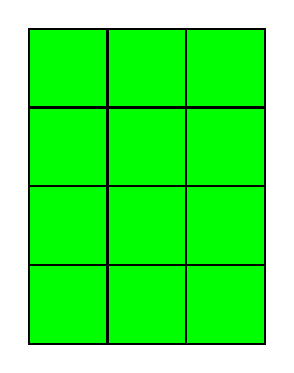
\begin{tikzpicture}
				[%%%%%%%%%%%%%%%%%%%%%%%%%%%%%%
				box/.style={rectangle,draw=black,thick, minimum size=1cm},
				]%%%%%%%%%%%%%%%%%%%%%%%%%%%%%%
				
				\foreach \x in {0,1,...,2}{
					\foreach \y in {0,1,...,3}
					\node[box, fill=red] at (\x,\y){};
				}
				
				
				\foreach \x in {0,...,2}{
					\foreach \y in {0,...,3} {
						\ifnumcomp{\x + (3 - \y)}{<}{5}{
							\node[box, fill=green] at (\x,\y){};
						}{};
					}
				}
				
				
			\end{tikzpicture}
		\end{center}
	\begin{center}
		(b)
	\end{center}
\end{minipage}
\caption{Taglio delle frequenze sulle diverse dimensioni dei blocchi}\label{fig:taglio}
\end{figure}

\section{Visualizzazione dei risultati}

Per mostrare meglio la compressione potremmo momentaneamente ignorare la conversione dei valori tramite la IDCT2. In figura\ref{fig:compression_values} viene mostrato il risultato ottenuto, dove è possibile osservare i coefficienti generati dalla DCT, i quali vengono successivamente tagliati per il valore di input scelto. In questo modo, ogni blocco conterrà dati diversi da 0 solo nella parte superiore del taglio, evidenziata anche graficamente dalla distribuzione del colore bianco nei singoli blocchi. Infatti tale tonalità rappresenta un valore elevato del coefficiente presente nella matrice, mentre le zone nere, rappresentano i valori che sono stati impostati a 0 dal taglio. Al fine di rendere migliore la visualizzazione, è stato temporaneamente modificato lo scaling delle DCT.

\begin{figure}[h]
	\centering
	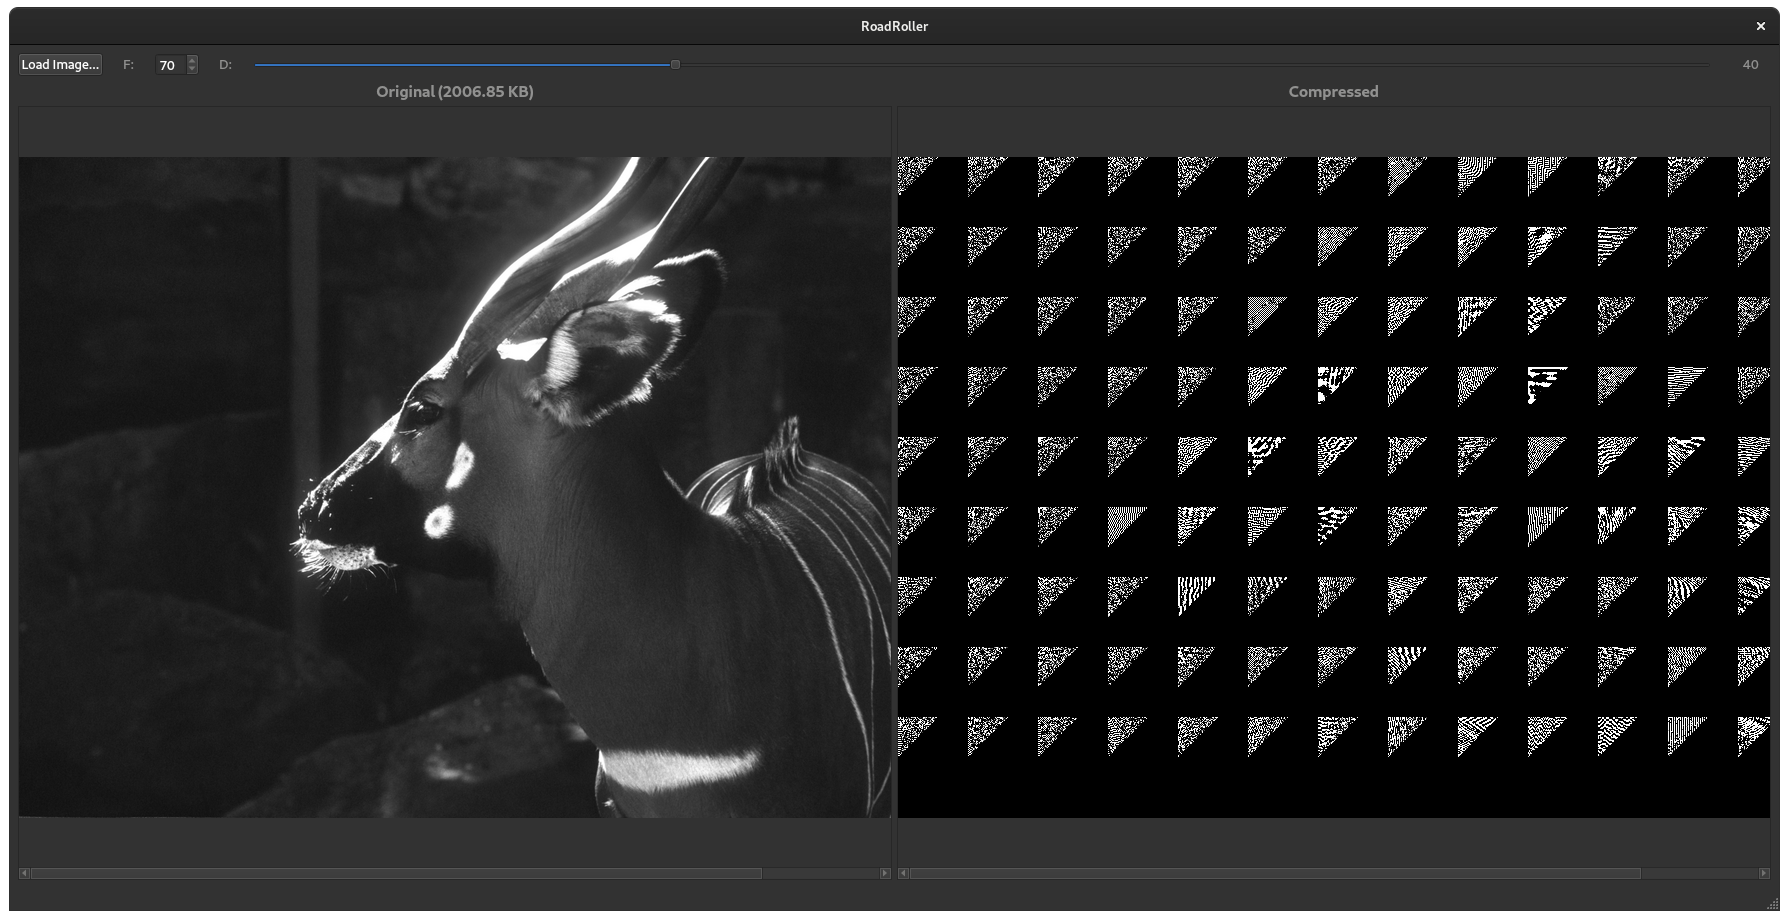
\includegraphics[width=1\linewidth]{figures/qt_dct_values}
	\caption{Valori della DCT generati dalla compressione (a meno dello scaling). Si noti il taglio netto delle frequenze determinato dalla soglia $d$.}
	\label{fig:compression_values}
\end{figure}

\subsection{Fenomeno di Gibbs}

Scegliendo un'elevata dimensione dei blocchi si rende particolarmente visibile il fenomeno di Gibbs, mostrato in Figura \ref{fig:gibbs}. La sua presenza tende ad essere più fastidiosa con blocchi grandi perché è più probabile che, all'aumentare di $F$, aumenta lo spazio all'interno del quale le basse frequenze cercano di compensare la carenza di quelle alte per rappresentare i cambiamenti repentini del tono di grigio presenti nel blocco stesso.

Nelle Figure \ref{fig:dct_values_on_gibbs} e \ref{fig:last_dct_values_gibbs} sono rappresentati rispettivamente l'intero istogramma del blocco mostrato in Figura \ref{fig:gibbs} e un suo zoom sulle ultime $50 \times 50$ frequenze. Nonostante la presenza di basse frequenze sia decisamente maggiore di quella delle alte frequenze, sono proprio quest'ultime che sono in grado di rappresentare al meglio i dettagli e, quindi, anche il bordo superiore della testa del cervo. Al momento del taglio, con un valore di $d$ basso, queste spariscono del tutto e non è, quindi, più possibile mostrare il cambiamento netto dell'immagine originale.

In contrasto, la Figura \ref{fig:gibbs_small} mostra come, la dimensione contenuta dei blocchi (in questo caso, $8 \times 8$), sia sufficiente al fine di limitare il fenomeno a piccolissime aree dell'immagine, rendendolo quasi impercettibile.

\begin{figure}[h]
	\centering
	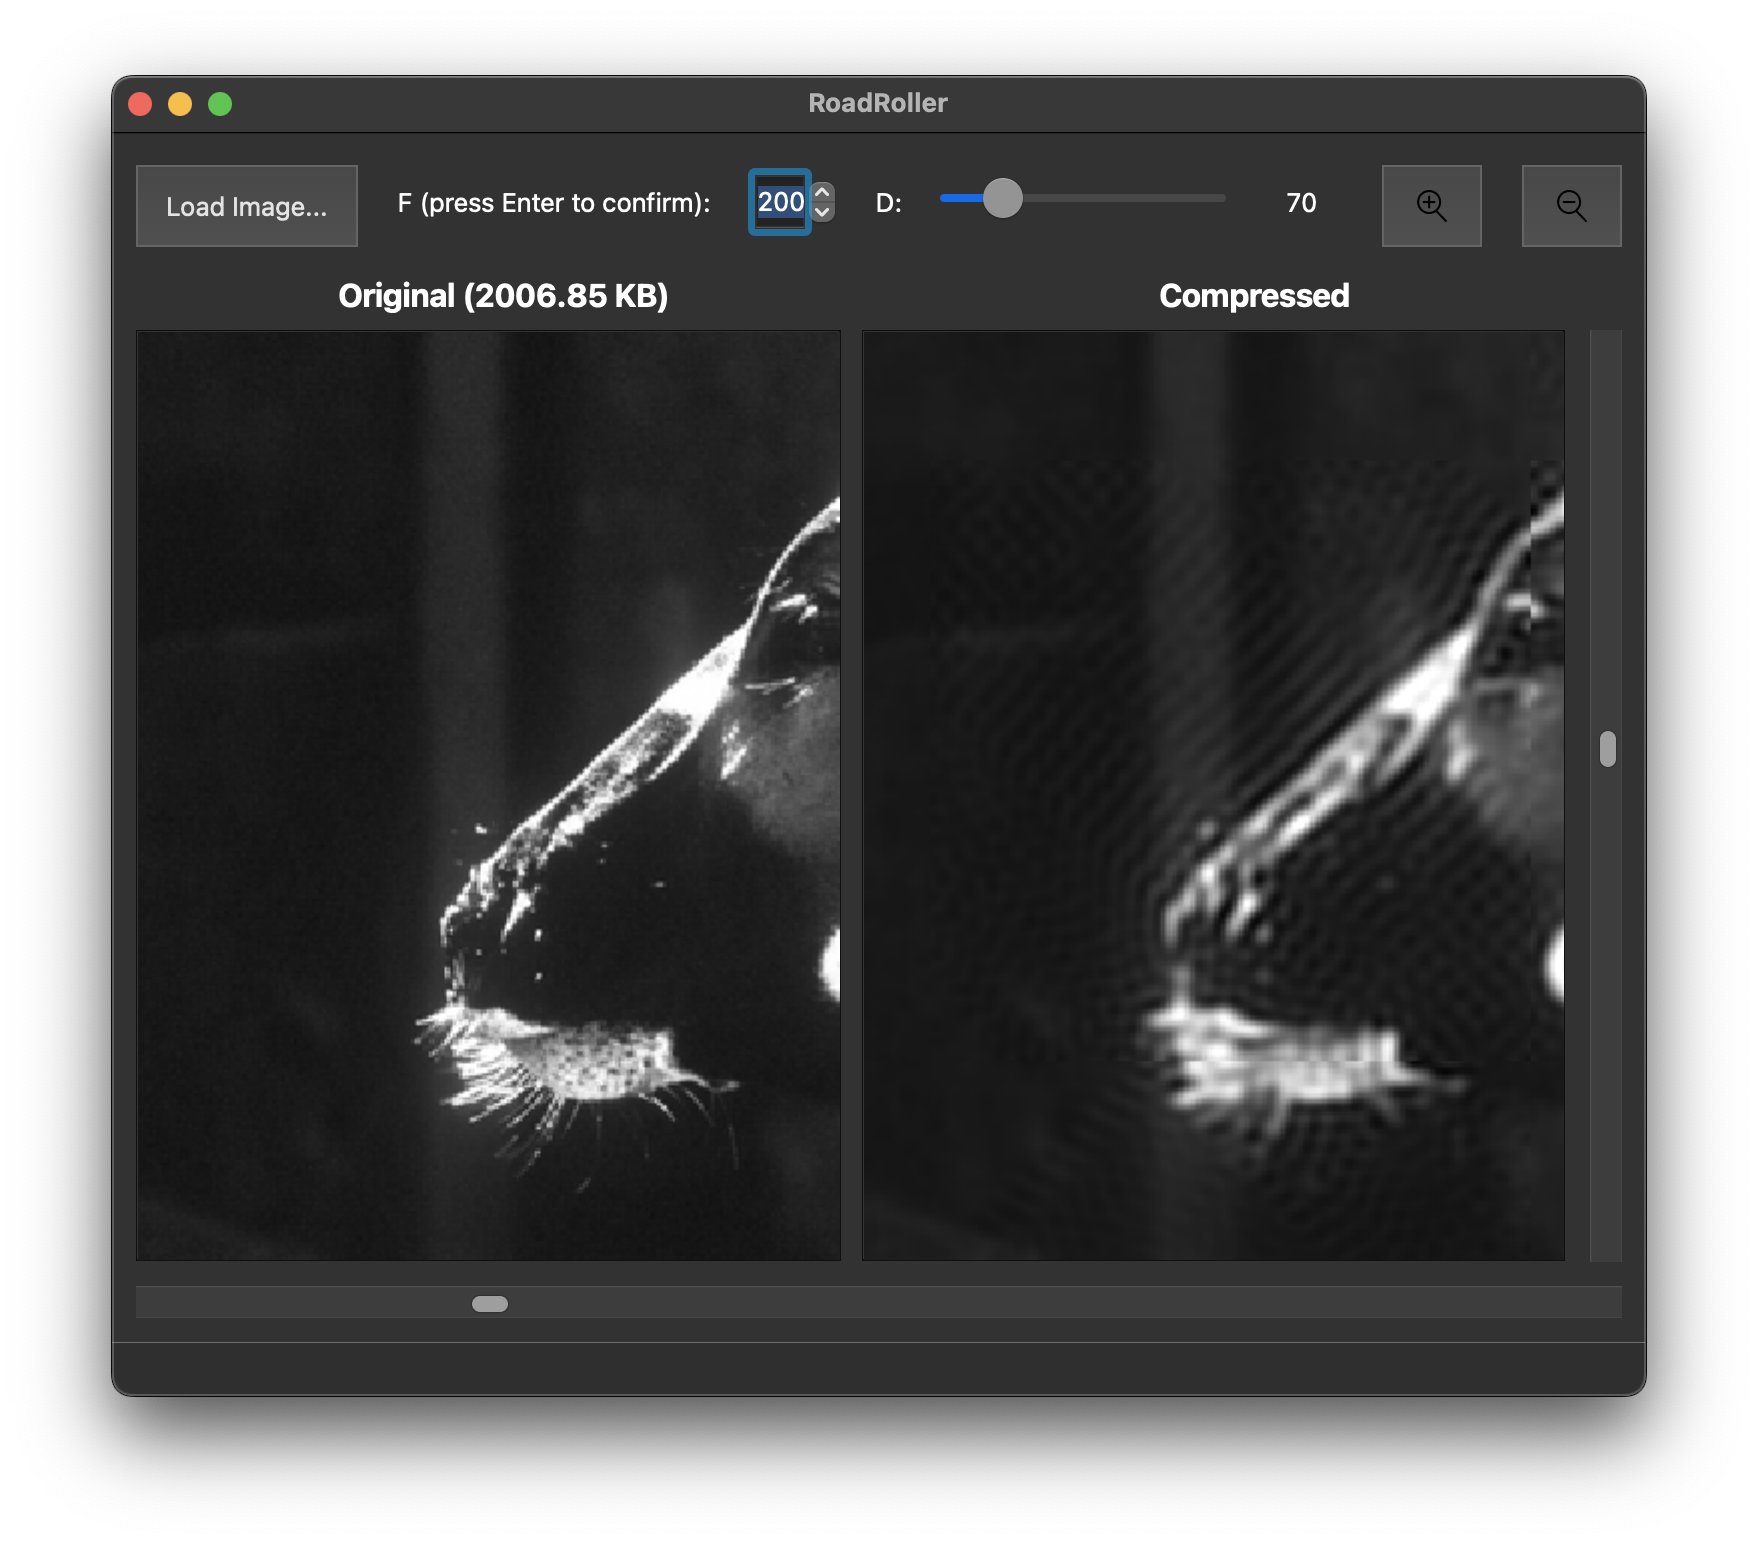
\includegraphics[width=1\linewidth]{figures/gibbs_phenomenon}
	\caption{Fenomeno di Gibbs su un blocco}
	\label{fig:gibbs}
\end{figure}

\begin{figure}[h]
	\centering
	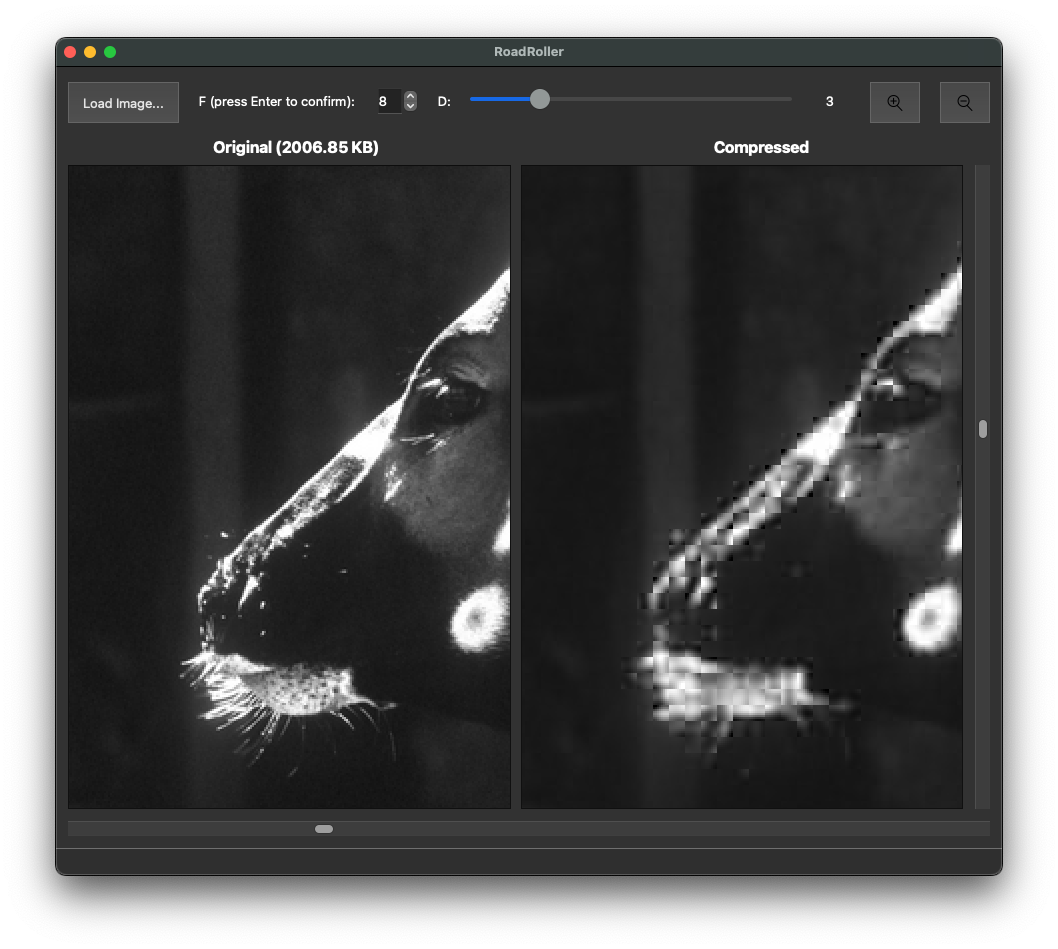
\includegraphics[width=1\linewidth]{figures/gibbs_small}
	\caption{Mitigazione del fenomeno di Gibbs sull'area dell'immagine mostrata in figura \ref{fig:gibbs}}.
	\label{fig:gibbs_small}
\end{figure}


\begin{figure}
	\centering
	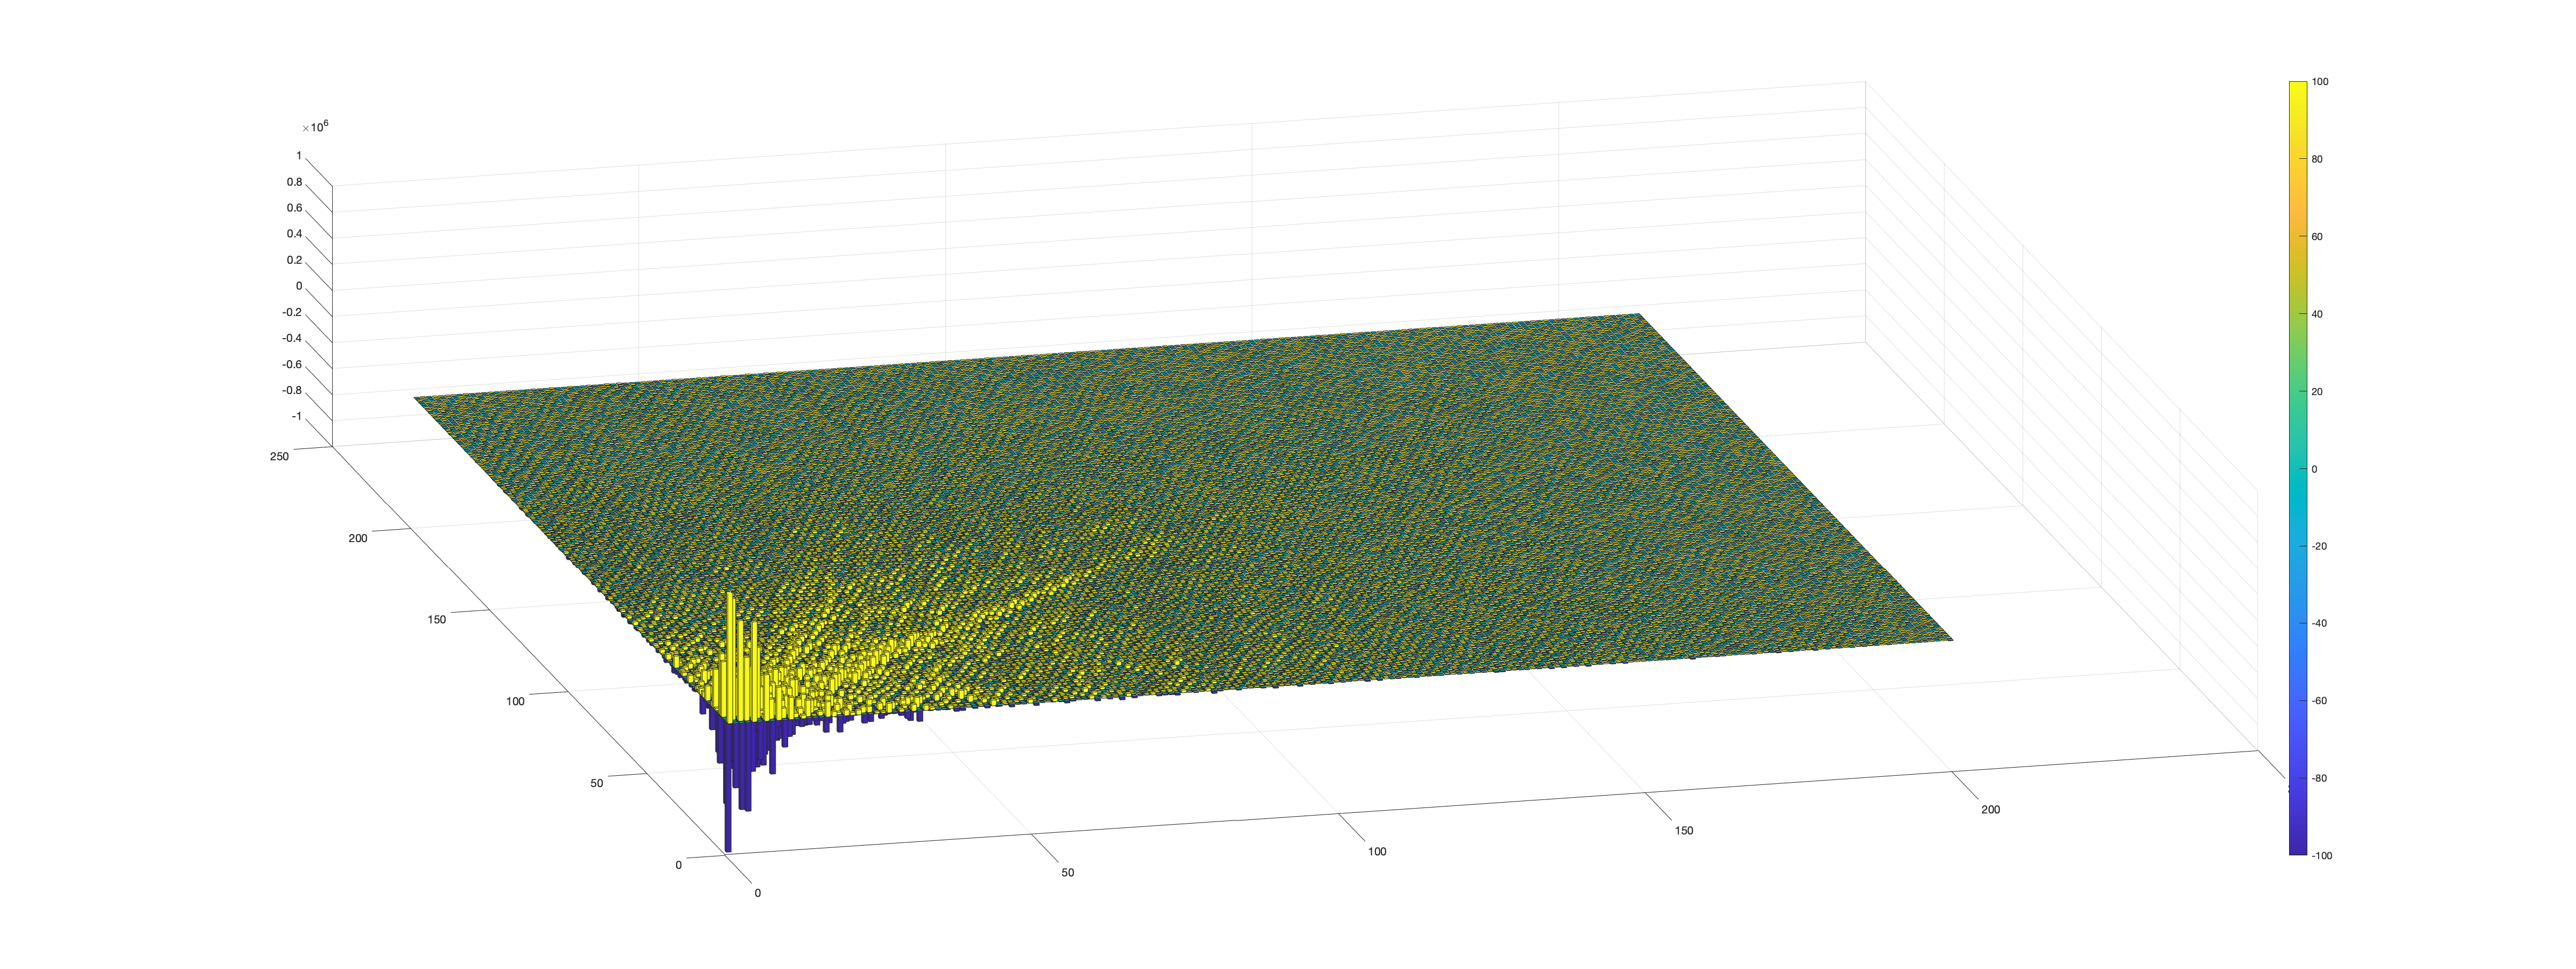
\includegraphics[width=1\linewidth]{figures/dct_values_3d.eps}
	\caption{Coefficienti DCT nel blocco mostrato in Figura \ref{fig:gibbs}}
	\label{fig:dct_values_on_gibbs}
\end{figure}

\begin{figure}
	\centering
	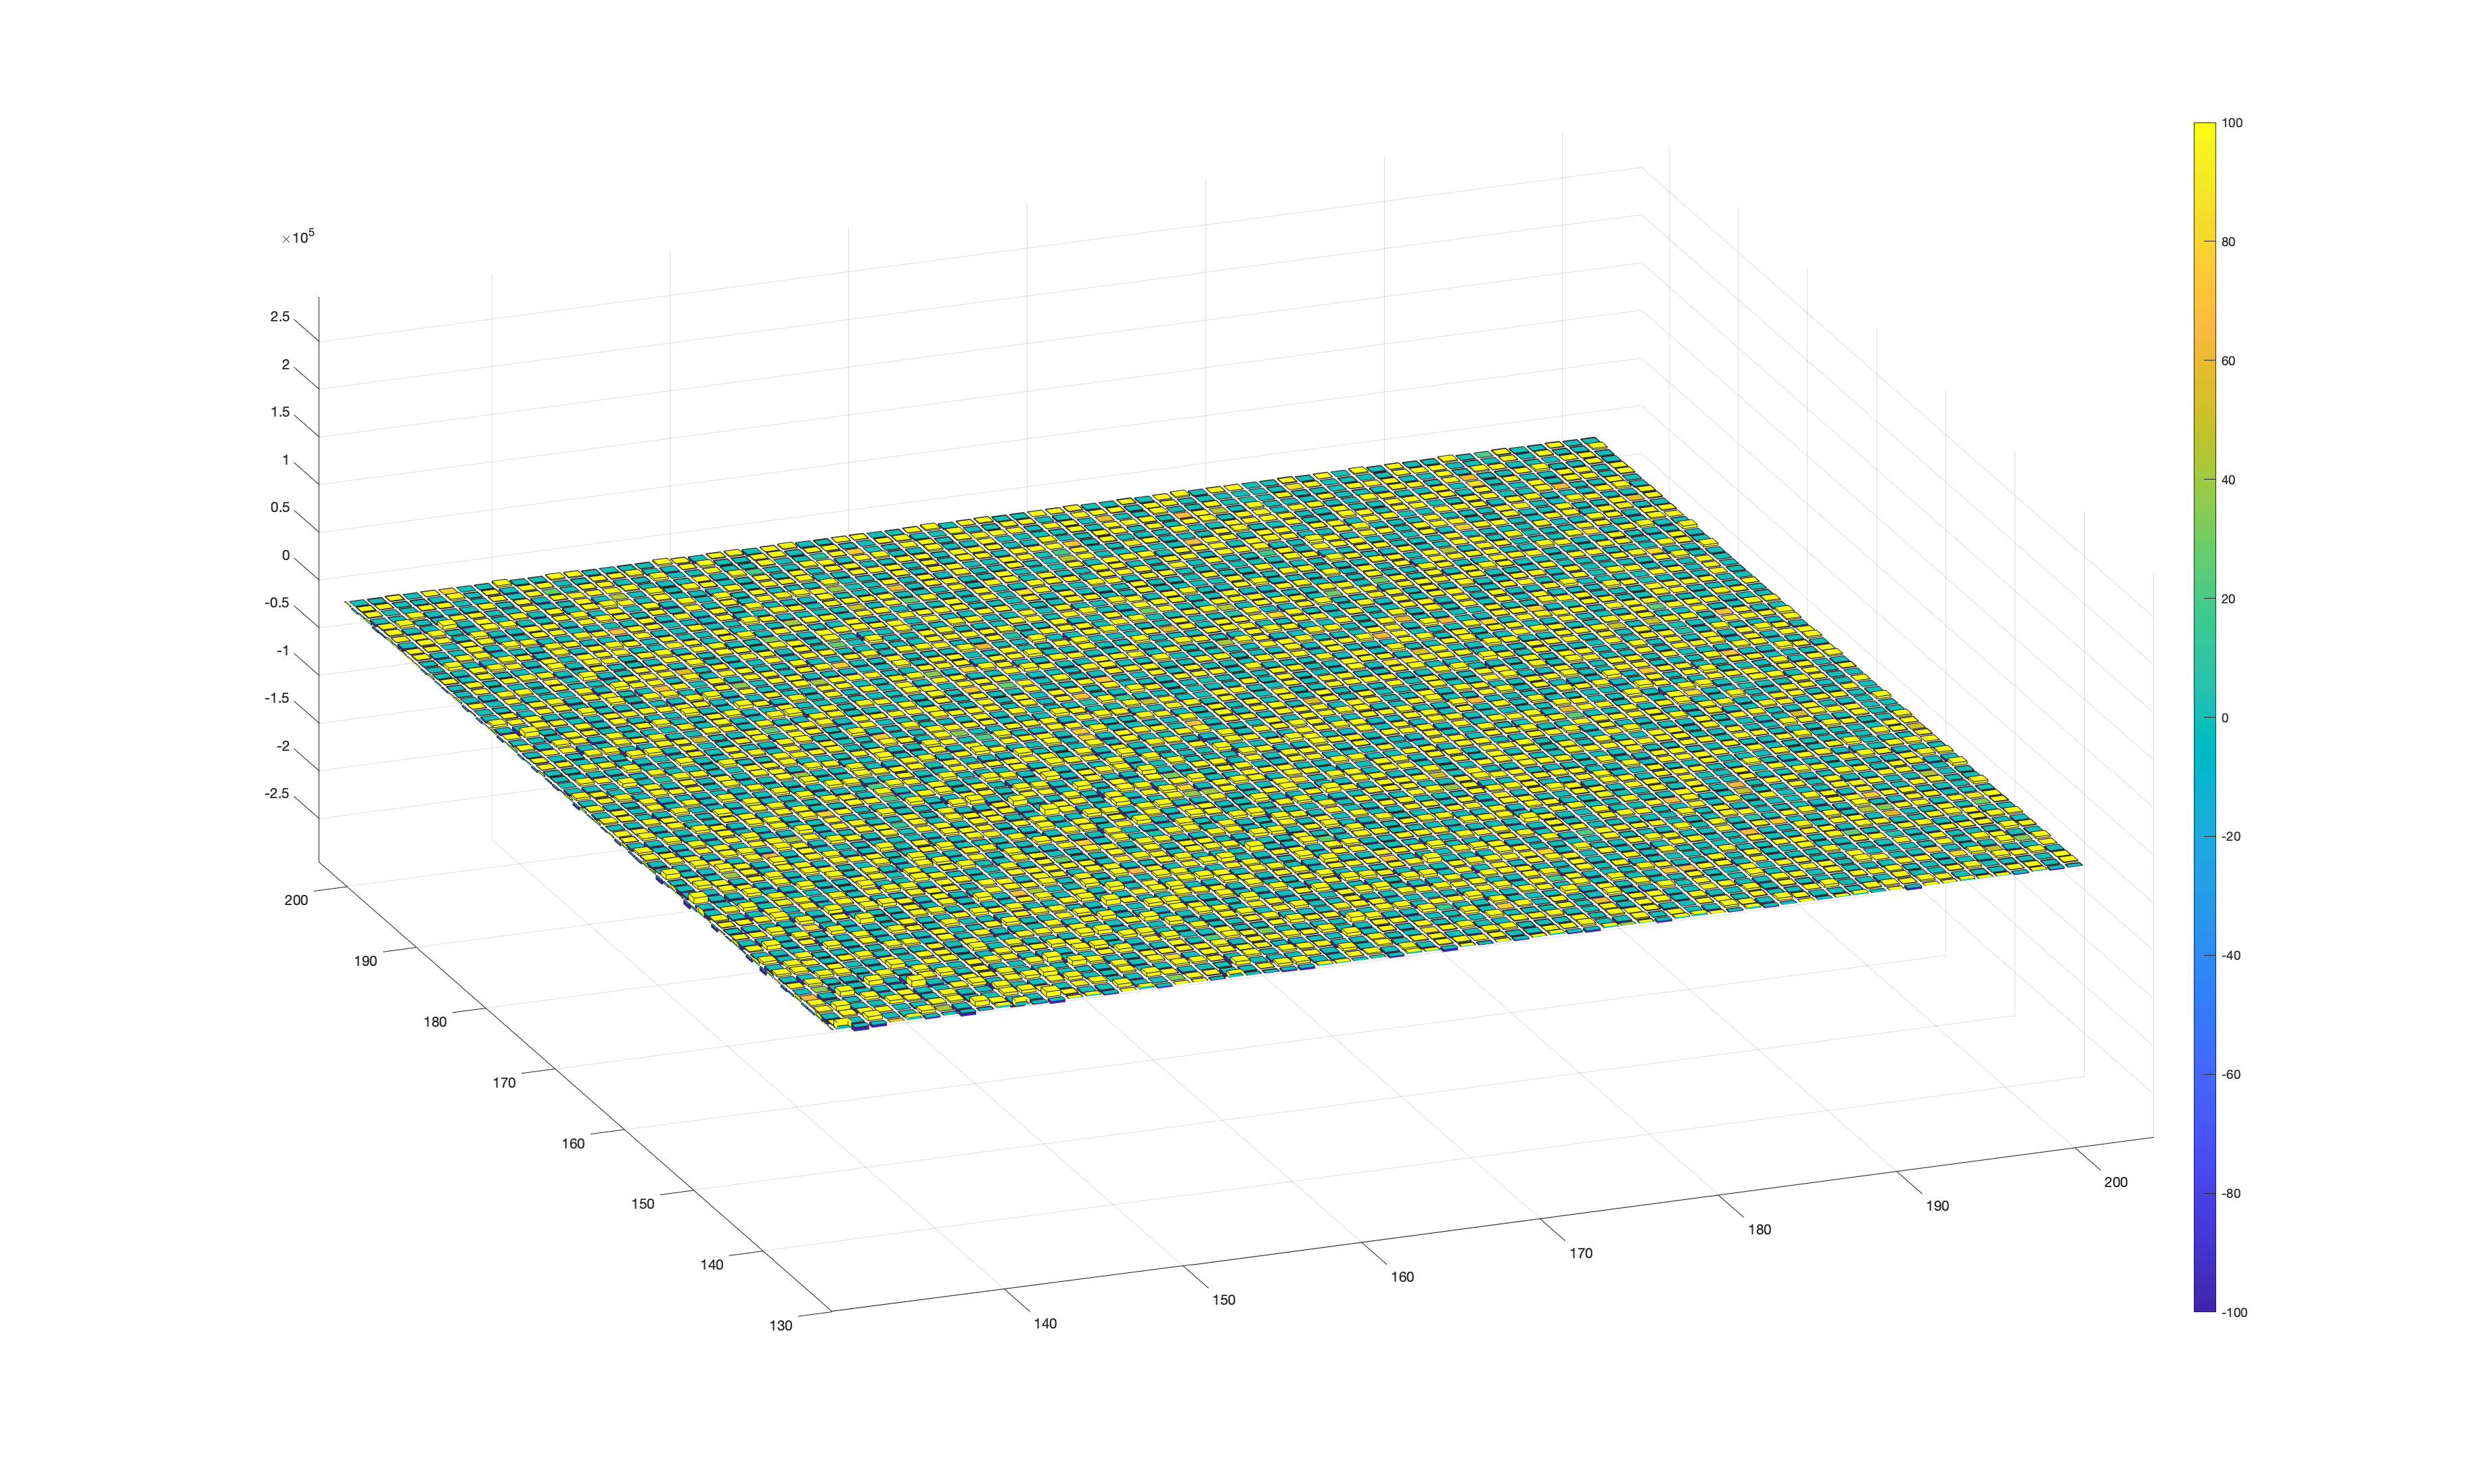
\includegraphics[width=1\linewidth]{figures/last_dct_values.eps}

	\caption{Ultimi 50 x 50 coefficienti della DCT relativi alla Figura \ref{fig:dct_values_on_gibbs}}
	\label{fig:last_dct_values_gibbs}
\end{figure}
\FloatBarrier

\subsection{DCT sui blocchi a margine}
Facendo qualche esperimento sulle immagini, specialmente quelle a quadrati bianchi e neri, abbiamo notato fondamentalmente due cose:
\begin{enumerate}
	\item Quando la dimensione dei blocchi è relativamente contenuta, la compressione risulta uniforme anche se i blocchi non sono della stessa dimensione di quelli interni;
	\item Nel momento in cui la compressione ha una soglia di taglio bassa e la dimensione del blocco diventa immensa (ad esempio, quasi tutta l'immagine) il risultato della compressione è molto diverso tra la parte interna dell'immagine e quella sui margini. Tuttavia, queesta differenza sparisce nel momento in cui si alza leggermente la soglia di taglio dei valori.
\end{enumerate}
Le due osservazioni sono evidenziate dalle Figure \ref{fig:border_small} e \ref{fig:border_big}. Riteniamo che questo metodo di gestione dei margini funzioni meglio quando i rapporti tra la larghezza e l'altezza di una singolo blocco non sono esageratamente alti,  mentre, nel caso in cui questi lo siano, è necessario un valore di $d$ più alto per arginare il problema. Pensiamo che il motivo principale sia questo perché, osservando l'ultimo blocco in basso a destra nella Figura \ref{fig:border_big}, si può notare che ha una forma quadrata e la sua compressione sia risultata molto più uniforme al resto dell'immagine rispetto ai due lungo i lati.


\begin{figure}
	\centering
	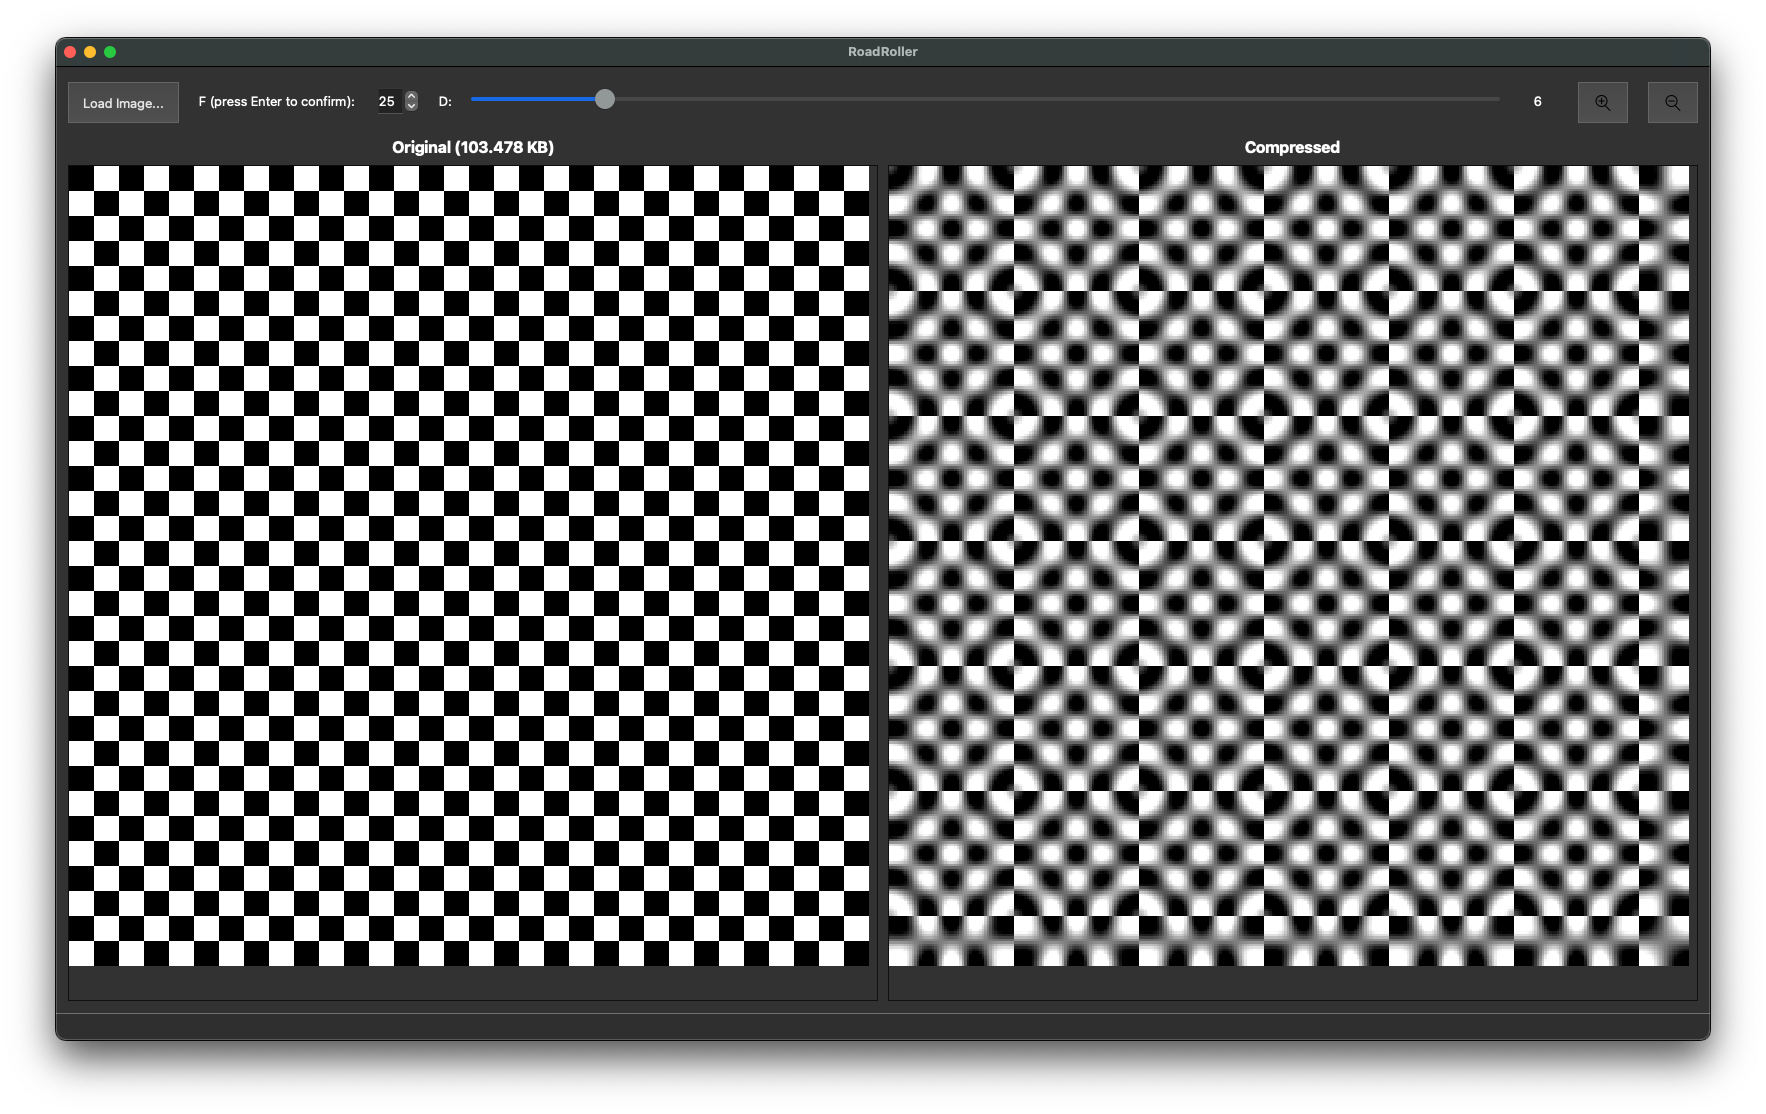
\includegraphics[width=0.7\linewidth]{figures/border_small}
	\caption{Compressione dell'immagine "320x320" con $F=25$ e $d=6$}
	\label{fig:border_small}
\end{figure}

\begin{figure}
	\centering
	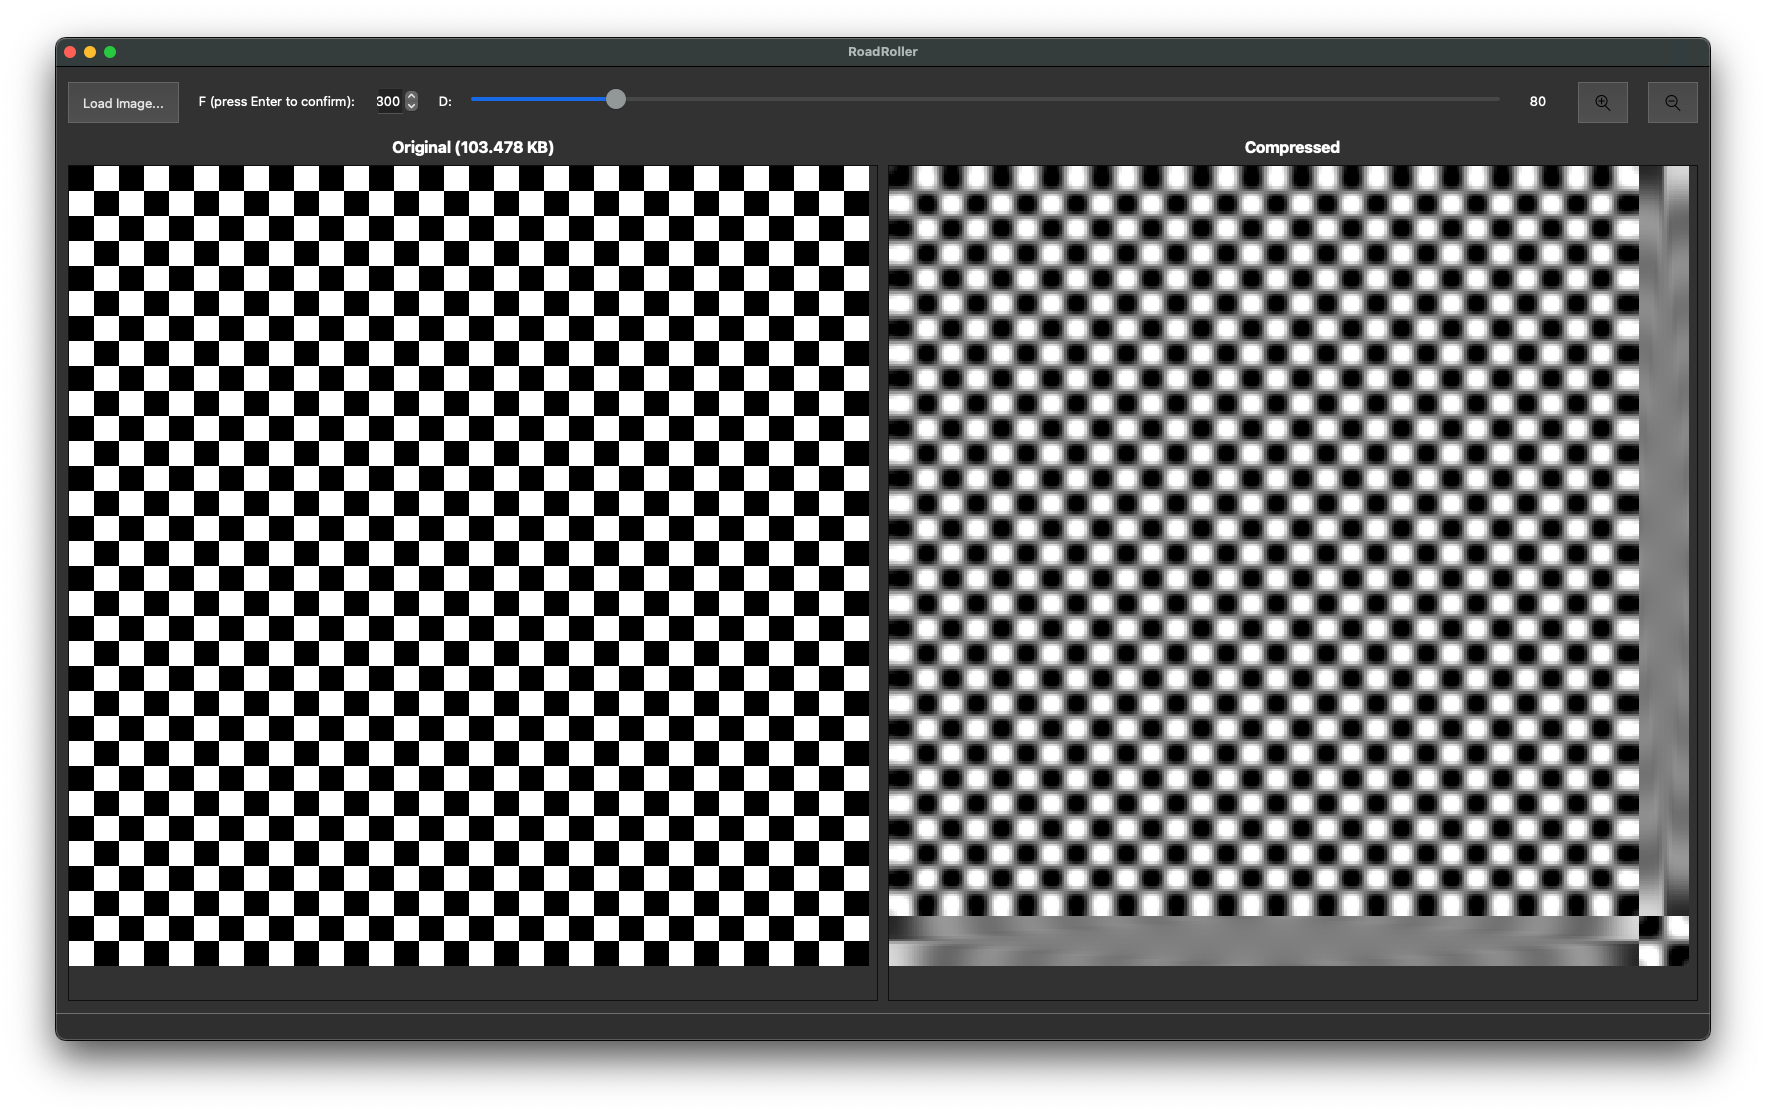
\includegraphics[width=0.7\linewidth]{figures/border_big}
	
	\caption{Compressione dell'immagine "320x320" con $F=300$ e $d=80$}
	\label{fig:border_big}
\end{figure}